\documentclass{article}\usepackage[]{graphicx}\usepackage[]{color}
%% maxwidth is the original width if it is less than linewidth
%% otherwise use linewidth (to make sure the graphics do not exceed the margin)
\makeatletter
\def\maxwidth{ %
  \ifdim\Gin@nat@width>\linewidth
    \linewidth
  \else
    \Gin@nat@width
  \fi
}
\makeatother

\definecolor{fgcolor}{rgb}{0.345, 0.345, 0.345}
\newcommand{\hlnum}[1]{\textcolor[rgb]{0.686,0.059,0.569}{#1}}%
\newcommand{\hlstr}[1]{\textcolor[rgb]{0.192,0.494,0.8}{#1}}%
\newcommand{\hlcom}[1]{\textcolor[rgb]{0.678,0.584,0.686}{\textit{#1}}}%
\newcommand{\hlopt}[1]{\textcolor[rgb]{0,0,0}{#1}}%
\newcommand{\hlstd}[1]{\textcolor[rgb]{0.345,0.345,0.345}{#1}}%
\newcommand{\hlkwa}[1]{\textcolor[rgb]{0.161,0.373,0.58}{\textbf{#1}}}%
\newcommand{\hlkwb}[1]{\textcolor[rgb]{0.69,0.353,0.396}{#1}}%
\newcommand{\hlkwc}[1]{\textcolor[rgb]{0.333,0.667,0.333}{#1}}%
\newcommand{\hlkwd}[1]{\textcolor[rgb]{0.737,0.353,0.396}{\textbf{#1}}}%
\let\hlipl\hlkwb

\usepackage{framed}
\makeatletter
\newenvironment{kframe}{%
 \def\at@end@of@kframe{}%
 \ifinner\ifhmode%
  \def\at@end@of@kframe{\end{minipage}}%
  \begin{minipage}{\columnwidth}%
 \fi\fi%
 \def\FrameCommand##1{\hskip\@totalleftmargin \hskip-\fboxsep
 \colorbox{shadecolor}{##1}\hskip-\fboxsep
     % There is no \\@totalrightmargin, so:
     \hskip-\linewidth \hskip-\@totalleftmargin \hskip\columnwidth}%
 \MakeFramed {\advance\hsize-\width
   \@totalleftmargin\z@ \linewidth\hsize
   \@setminipage}}%
 {\par\unskip\endMakeFramed%
 \at@end@of@kframe}
\makeatother

\definecolor{shadecolor}{rgb}{.97, .97, .97}
\definecolor{messagecolor}{rgb}{0, 0, 0}
\definecolor{warningcolor}{rgb}{1, 0, 1}
\definecolor{errorcolor}{rgb}{1, 0, 0}
\newenvironment{knitrout}{}{} % an empty environment to be redefined in TeX

\usepackage{alltt}
\usepackage{graphicx, color, framed, alltt,fullpage}
\IfFileExists{upquote.sty}{\usepackage{upquote}}{}
\begin{document}

\setcounter{section}{5}
\setcounter{page}{5}
\section{Walkthrough with examples in R}

\subsection{Getting the variables}
When performing this analysis on a set of data, we start with the autocorrelation functions of the two channels in each image, and labels of whether these images are bijels or not.

\begin{knitrout}
\definecolor{shadecolor}{rgb}{0.969, 0.969, 0.969}\color{fgcolor}\begin{kframe}
\begin{verbatim}
##      Sample.Number Bijel            ACF_1              ACF_2
## 19              19     n list(ACF_liquid) list(ACF_particle)
## 20i            20i     y list(ACF_liquid) list(ACF_particle)
## 20ii          20ii     y list(ACF_liquid) list(ACF_particle)
## 21              21     n list(ACF_liquid) list(ACF_particle)
## 22i            22i     n list(ACF_liquid) list(ACF_particle)
## 22ii          22ii     n list(ACF_liquid) list(ACF_particle)
\end{verbatim}
\end{kframe}
\end{knitrout}

We then need to turn these functions into a set of single-valued variables that describe features that may separate bijels from non-bijels, such as:

\begin{itemize}
\item The gradient of the particle channel autocorrelation function
\end{itemize}


\begin{knitrout}
\definecolor{shadecolor}{rgb}{0.969, 0.969, 0.969}\color{fgcolor}\begin{kframe}
\begin{alltt}
\hlstd{r} \hlkwb{<-} \hlkwd{c}\hlstd{(}\hlnum{1}\hlopt{:}\hlnum{256}\hlstd{)}
\hlstd{num_points} \hlkwb{<-} \hlkwd{length}\hlstd{(exp_Data}\hlopt{$}\hlstd{Sample.Number)}
\hlstd{y} \hlkwb{<-} \hlstd{exp_Data}\hlopt{$}\hlstd{Autocorrelation.Particle[}\hlnum{1}\hlopt{:}\hlnum{20}\hlstd{]}
\hlstd{lineFits} \hlkwb{<-} \hlkwd{lapply}\hlstd{(}\hlnum{1}\hlopt{:}\hlstd{num_points,}
                  \hlkwa{function}\hlstd{(}\hlkwc{n}\hlstd{)} \hlkwd{lm}\hlstd{(}\hlkwd{unlist}\hlstd{(y[n,])} \hlopt{~} \hlstd{r[}\hlnum{1}\hlopt{:}\hlnum{20}\hlstd{]))}
\hlstd{lineCoeffs} \hlkwb{<-} \hlkwd{lapply}\hlstd{(lineFits,}
                     \hlkwa{function}\hlstd{(}\hlkwc{m}\hlstd{) m}\hlopt{$}\hlstd{coefficients)}
\hlstd{lineGradients} \hlkwb{<-} \hlkwd{lapply} \hlstd{(}\hlnum{1}\hlopt{:}\hlstd{num_points,}
                          \hlkwa{function}\hlstd{(}\hlkwc{p}\hlstd{)} \hlkwd{unname}\hlstd{(lineCoeffs[[p]][}\hlnum{2}\hlstd{]))}
\hlstd{exp_Data}\hlopt{$}\hlstd{Particle.Gradients.20} \hlkwb{<-} \hlkwd{unlist}\hlstd{(lineGradients)}


\hlkwd{library}\hlstd{(ggplot2)}
\hlkwd{ggplot}\hlstd{(exp_Data,}
       \hlkwd{aes}\hlstd{(}\hlkwc{x}\hlstd{=}\hlkwd{as.factor}\hlstd{(Bijel),} \hlkwc{y}\hlstd{=Particle.Gradients.20,}
           \hlkwc{fill}\hlstd{=Bijel))} \hlopt{+}
       \hlkwd{geom_boxplot}\hlstd{(}\hlkwc{alpha}\hlstd{=}\hlnum{0.3}\hlstd{)} \hlopt{+}
       \hlkwd{geom_jitter}\hlstd{(}\hlkwc{alpha}\hlstd{=}\hlnum{0.5}\hlstd{)} \hlopt{+}
       \hlkwd{xlab}\hlstd{(}\hlstr{"Bijel?"}\hlstd{)} \hlopt{+} \hlkwd{ylab}\hlstd{(}\hlstr{"Gradient"}\hlstd{)} \hlopt{+}
       \hlkwd{ggtitle}\hlstd{(}\hlstr{"Gradient of first 20 points of particle ACF"}\hlstd{)} \hlopt{+}
       \hlkwd{theme}\hlstd{(}\hlkwc{plot.title} \hlstd{=} \hlkwd{element_text}\hlstd{(}\hlkwc{hjust} \hlstd{=} \hlnum{0.5}\hlstd{))}
\end{alltt}
\end{kframe}
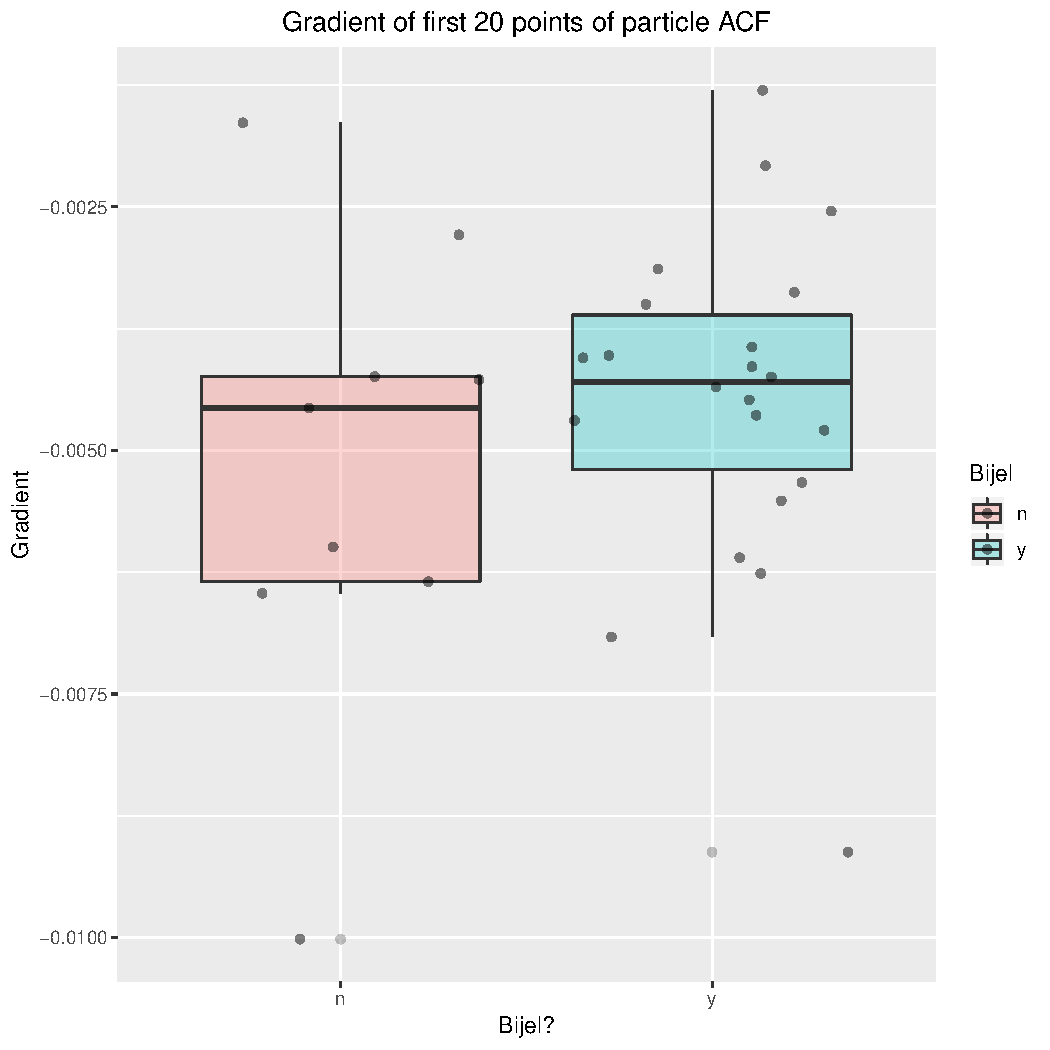
\includegraphics[width=\maxwidth]{figure/unnamed-chunk-2-1} 
\begin{kframe}\begin{alltt}
\hlstd{y2} \hlkwb{<-} \hlstd{exp_Data}\hlopt{$}\hlstd{Autocorrelation.Particle[}\hlnum{1}\hlopt{:}\hlnum{10}\hlstd{]}
\hlstd{lineFits2} \hlkwb{<-} \hlkwd{lapply}\hlstd{(}\hlnum{1}\hlopt{:}\hlstd{num_points,}
                    \hlkwa{function}\hlstd{(}\hlkwc{n}\hlstd{)} \hlkwd{lm}\hlstd{(}\hlkwd{unlist}\hlstd{(y2[n,])} \hlopt{~} \hlstd{r[}\hlnum{1}\hlopt{:}\hlnum{10}\hlstd{]))}
\hlstd{lineCoeffs2} \hlkwb{<-} \hlkwd{lapply}\hlstd{(lineFits2,}
                      \hlkwa{function}\hlstd{(}\hlkwc{m}\hlstd{) m}\hlopt{$}\hlstd{coefficients)}
\hlstd{lineGradients2} \hlkwb{<-} \hlkwd{lapply} \hlstd{(}\hlnum{1}\hlopt{:}\hlstd{num_points,}
                          \hlkwa{function}\hlstd{(}\hlkwc{p}\hlstd{)} \hlkwd{unname}\hlstd{(lineCoeffs2[[p]][}\hlnum{2}\hlstd{]))}
\hlstd{exp_Data}\hlopt{$}\hlstd{Particle.Gradients.10} \hlkwb{<-} \hlkwd{unlist}\hlstd{(lineGradients2)}

\hlkwd{ggplot}\hlstd{(exp_Data,}
       \hlkwd{aes}\hlstd{(}\hlkwc{x}\hlstd{=}\hlkwd{as.factor}\hlstd{(Bijel),} \hlkwc{y}\hlstd{=Particle.Gradients.10,}
           \hlkwc{fill}\hlstd{=Bijel))} \hlopt{+}
       \hlkwd{geom_boxplot}\hlstd{(}\hlkwc{alpha}\hlstd{=}\hlnum{0.3}\hlstd{)} \hlopt{+}
       \hlkwd{geom_jitter}\hlstd{(}\hlkwc{alpha}\hlstd{=}\hlnum{0.5}\hlstd{)} \hlopt{+}
       \hlkwd{xlab}\hlstd{(}\hlstr{"Bijel?"}\hlstd{)} \hlopt{+} \hlkwd{ylab}\hlstd{(}\hlstr{"Gradient"}\hlstd{)} \hlopt{+}
       \hlkwd{ggtitle}\hlstd{(}\hlstr{"Gradient of first 10 points of particle ACF"}\hlstd{)} \hlopt{+}
       \hlkwd{theme}\hlstd{(}\hlkwc{plot.title} \hlstd{=} \hlkwd{element_text}\hlstd{(}\hlkwc{hjust} \hlstd{=} \hlnum{0.5}\hlstd{))}
\end{alltt}
\end{kframe}
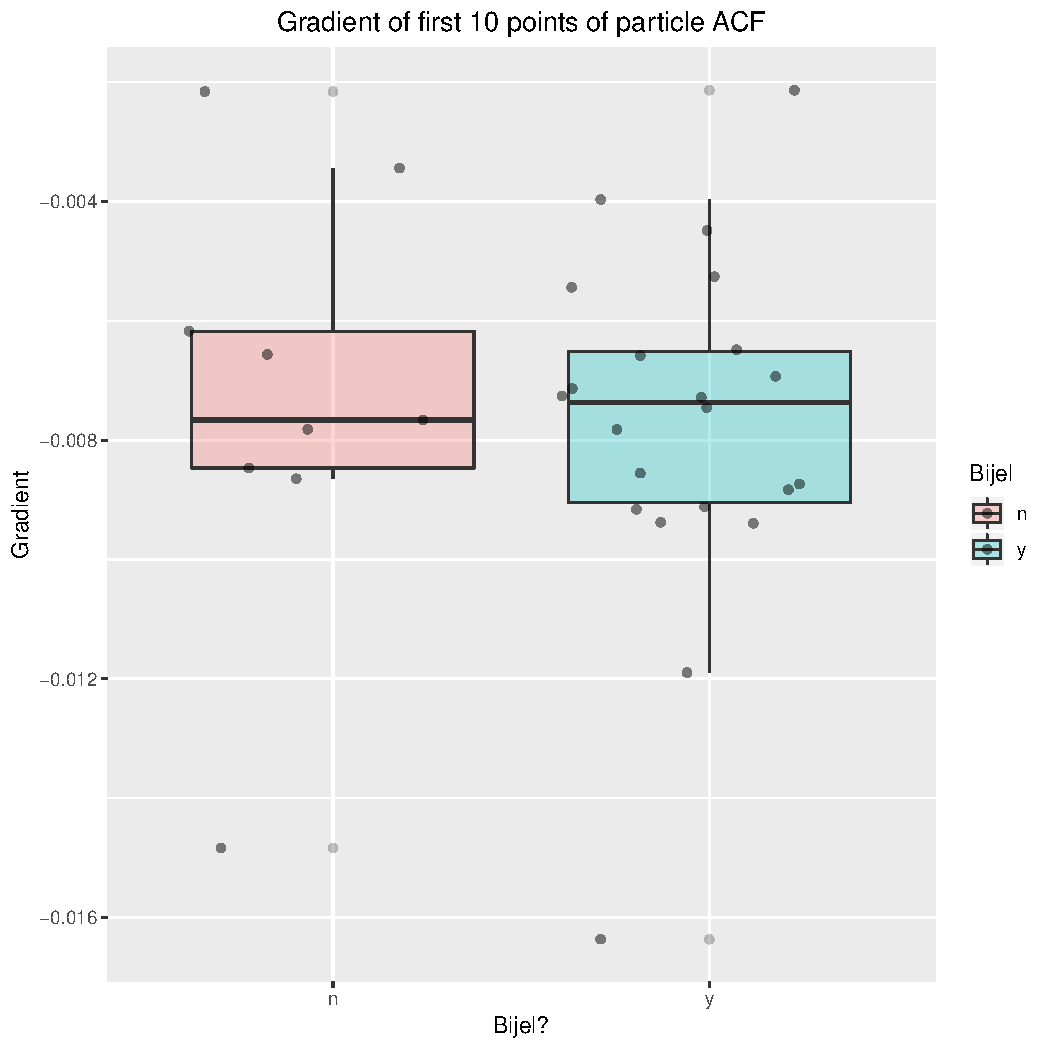
\includegraphics[width=\maxwidth]{figure/unnamed-chunk-2-2} 

\end{knitrout}

\begin{itemize}
\item The position of the first turning point in the liquid channel autocorrelation function
\end{itemize}

\begin{knitrout}
\definecolor{shadecolor}{rgb}{0.969, 0.969, 0.969}\color{fgcolor}\begin{kframe}
\begin{alltt}
\hlkwd{library}\hlstd{(pastecs)}
\hlstd{liquidTurns} \hlkwb{<-} \hlkwd{lapply}\hlstd{(}\hlnum{1}\hlopt{:}\hlstd{num_points,}
                      \hlkwa{function}\hlstd{(}\hlkwc{y}\hlstd{)} \hlkwd{turnpoints}\hlstd{(}\hlkwd{unlist}\hlstd{(}
                        \hlstd{exp_Data}\hlopt{$}\hlstd{Autocorrelation.Liquid[y,])))}
\hlstd{firstTurn} \hlkwb{<-} \hlkwd{lapply}\hlstd{(}\hlnum{1}\hlopt{:}\hlstd{num_points,}
                    \hlkwa{function}\hlstd{(}\hlkwc{y}\hlstd{) liquidTurns[[y]]}\hlopt{$}\hlstd{tppos[}\hlnum{1}\hlstd{])}
\hlstd{exp_Data}\hlopt{$}\hlstd{Liquid.First.Turn} \hlkwb{<-} \hlkwd{unlist}\hlstd{(firstTurn)}

\hlkwd{ggplot}\hlstd{(exp_Data,}
       \hlkwd{aes}\hlstd{(}\hlkwc{x}\hlstd{=}\hlkwd{as.factor}\hlstd{(Bijel),} \hlkwc{y}\hlstd{=Liquid.First.Turn,}
           \hlkwc{fill}\hlstd{=Bijel))} \hlopt{+}
       \hlkwd{geom_boxplot}\hlstd{(}\hlkwc{alpha}\hlstd{=}\hlnum{0.3}\hlstd{)} \hlopt{+}
       \hlkwd{geom_jitter}\hlstd{(}\hlkwc{alpha}\hlstd{=}\hlnum{0.5}\hlstd{)} \hlopt{+}
       \hlkwd{xlab}\hlstd{(}\hlstr{"Bijel?"}\hlstd{)} \hlopt{+} \hlkwd{ylab}\hlstd{(}\hlstr{"Position"}\hlstd{)} \hlopt{+}
       \hlkwd{ggtitle}\hlstd{(}\hlstr{"Position of first turning points of liquid ACF"}\hlstd{)}
\end{alltt}
\end{kframe}
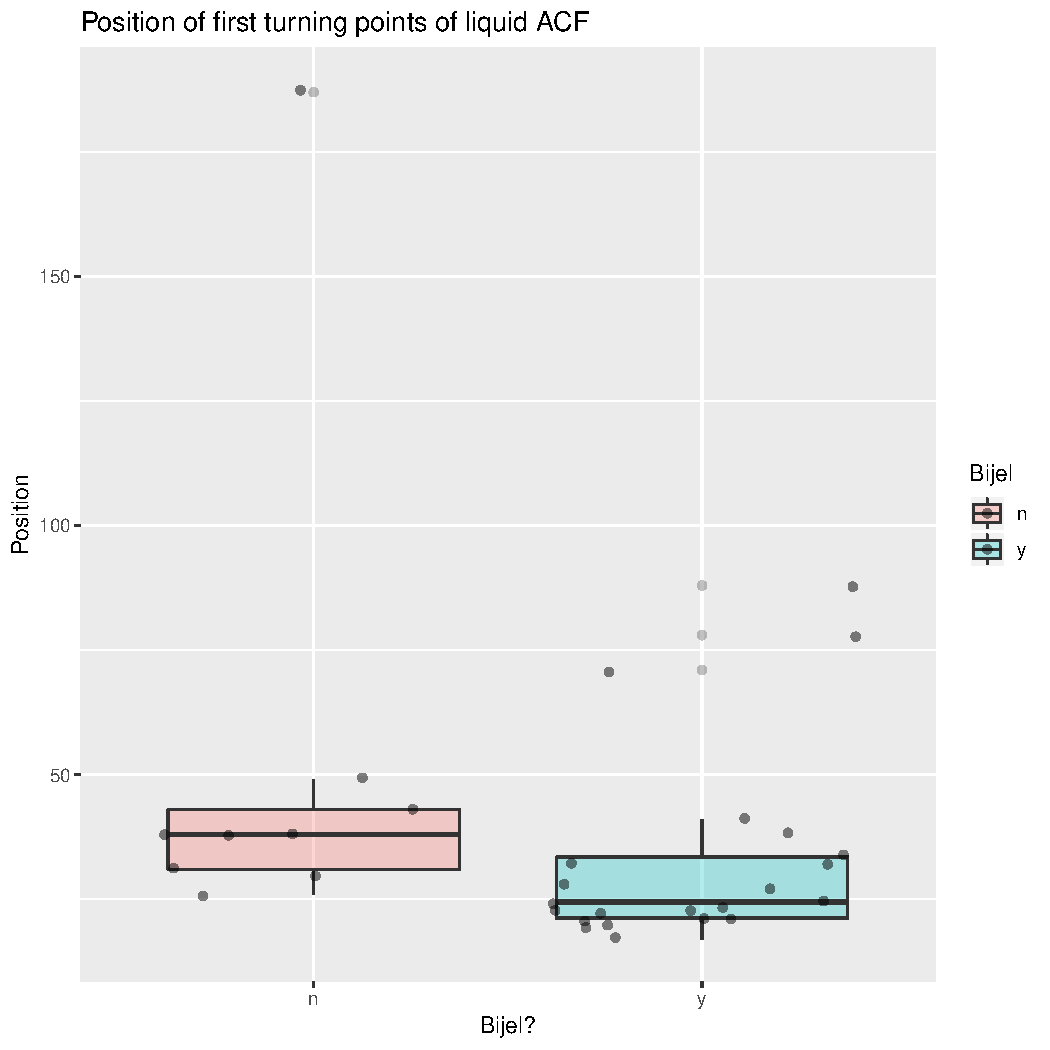
\includegraphics[width=\maxwidth]{figure/unnamed-chunk-3-1} 

\end{knitrout}

We have generated box-and-jitter plots to see how the distribution of these variables is dependent on whether or not the sample is a bijel.

Once we have these variables, we can apply a machine learning model to it in one of two ways: training the model on the data and testing via cross-validation, and testing a previously trained model on the new data.

\subsection{Training a model and testing with cross-validation}
Here we have chosen to train a k-nearest neighbours model with the three variables shown above, based on our experience with a previous set of data. This can be done very simply using the CARET package in R, which contains a number of widely-used machine learning algorithms as well as cross-validation capabilities. 

\begin{knitrout}
\definecolor{shadecolor}{rgb}{0.969, 0.969, 0.969}\color{fgcolor}\begin{kframe}
\begin{alltt}
\hlkwd{library}\hlstd{(caret)}
\end{alltt}


{\ttfamily\noindent\itshape\color{messagecolor}{\#\# Loading required package: lattice}}\begin{alltt}
\hlcom{# set up the data}
\hlkwd{attach}\hlstd{(exp_Data)}
\hlstd{dat}\hlkwb{=}\hlkwd{data.frame}\hlstd{(}
  \hlstd{Particle.Gradients.20,}
  \hlstd{Particle.Gradients.10,}
  \hlstd{Liquid.First.Turn,}
  \hlstd{Bijel)}

\hlcom{# set a random number seed for reproducability}
\hlkwd{set.seed}\hlstd{(}\hlnum{1234}\hlstd{)}

\hlcom{# define the cross-validation parameters:}
\hlcom{# here we use 10-fold cross-validation and repeat it 3 times}
\hlstd{trCtrl} \hlkwb{<-} \hlkwd{trainControl}\hlstd{(}
  \hlkwc{method} \hlstd{=} \hlstr{"repeatedcv"}\hlstd{,}
  \hlkwc{number} \hlstd{=} \hlnum{10}\hlstd{,}
  \hlkwc{repeats} \hlstd{=} \hlnum{3}\hlstd{)}

\hlstd{knnFit} \hlkwb{<-} \hlkwd{train}\hlstd{(Bijel}\hlopt{~}\hlstd{.,} \hlcom{# Bijel = output, other variables = input}
                \hlkwc{data}\hlstd{=dat,} \hlcom{# define the data}
                \hlkwc{method}\hlstd{=}\hlstr{"knn"}\hlstd{,} \hlcom{# choose the algorithm}
                \hlkwc{trControl}\hlstd{=trCtrl,} \hlcom{# cross-validation as above}
                \hlkwc{tuneLength}\hlstd{=}\hlnum{10}\hlstd{)}
\hlkwd{print}\hlstd{(knnFit)}
\end{alltt}
\begin{verbatim}
## k-Nearest Neighbors 
## 
## 31 samples
##  3 predictor
##  2 classes: 'n', 'y' 
## 
## No pre-processing
## Resampling: Cross-Validated (10 fold, repeated 3 times) 
## Summary of sample sizes: 28, 28, 28, 28, 28, 27, ... 
## Resampling results across tuning parameters:
## 
##   k   Accuracy   Kappa      
##    5  0.6611111   0.13928571
##    7  0.5611111  -0.01034483
##    9  0.6638889   0.19310345
##   11  0.7055556   0.22758621
##   13  0.7388889   0.25000000
##   15  0.7000000   0.00000000
##   17  0.7166667   0.00000000
##   19  0.7166667   0.00000000
##   21  0.7166667   0.00000000
##   23  0.7166667   0.00000000
## 
## Accuracy was used to select the optimal model using the largest value.
## The final value used for the model was k = 13.
\end{verbatim}
\end{kframe}
\end{knitrout}

%Cross-validation has been used to determine that the model performs best with $k=13$, and gives an error of around 16\%. This is similar to the result gained from the previous dataset, suggesting that the model is useful more generally than with just the system used to choose it.

%To apply a different algorithm to the same data, it is a simple case of changing the algorithm choice in the \verbatim{train()} function and/or changing the input variables. 

\subsection{Testing a trained model on new data}
If we have already trained a model, we can use it to classify new data. This is how the algorithm can be used as a tool to classify unlabelled data.



\begin{knitrout}
\definecolor{shadecolor}{rgb}{0.969, 0.969, 0.969}\color{fgcolor}\begin{kframe}
\begin{alltt}
\hlcom{# predict whether the data points are bijels or not}
\hlcom{# to do this, we have to omit the bijel label from the data}
\hlstd{bijel_pred} \hlkwb{=} \hlkwd{predict}\hlstd{(trainedKNN,} \hlkwc{newdata} \hlstd{= dat[,}\hlopt{-}\hlnum{4}\hlstd{])}
\hlstd{bijel_true} \hlkwb{=} \hlstd{dat[,}\hlnum{4}\hlstd{]}
\hlkwd{print}\hlstd{(}\hlkwd{data.frame}\hlstd{(bijel_pred,} \hlkwc{bijel_true}\hlstd{=bijel_true))}
\end{alltt}
\begin{verbatim}
##    bijel_pred bijel_true
## 1           y          n
## 2           y          y
## 3           y          y
## 4           y          n
## 5           y          n
## 6           y          n
## 7           y          y
## 8           y          y
## 9           y          n
## 10          y          n
## 11          y          y
## 12          y          y
## 13          y          n
## 14          n          n
## 15          n          n
## 16          n          y
## 17          y          y
## 18          y          y
## 19          y          y
## 20          y          y
## 21          y          y
## 22          y          y
## 23          y          y
## 24          y          y
## 25          n          y
## 26          n          y
## 27          y          y
## 28          n          y
## 29          y          y
## 30          n          y
## 31          y          y
\end{verbatim}
\end{kframe}
\end{knitrout}

We can now calculate the error rate, and also look at the results to see how many false positives, false negatives, etc. we have.

\begin{knitrout}
\definecolor{shadecolor}{rgb}{0.969, 0.969, 0.969}\color{fgcolor}\begin{kframe}
\begin{alltt}
\hlstd{success_count}\hlkwb{=}\hlkwd{length}\hlstd{(bijel_pred[bijel_pred}\hlopt{==}\hlstd{bijel_true])}
\hlstd{success_rate}\hlkwb{=}\hlstd{success_count}\hlopt{/}\hlkwd{length}\hlstd{(bijel_pred)}
\hlkwd{paste0}\hlstd{(}\hlstr{"Success rate: "}\hlstd{,}\hlkwd{round}\hlstd{(}\hlnum{100}\hlopt{*}\hlstd{success_rate),}\hlstr{"%"}\hlstd{)}
\end{alltt}
\begin{verbatim}
## [1] "Success rate: 61%"
\end{verbatim}
\begin{alltt}
\hlkwd{library}\hlstd{(gmodels)}
\hlkwd{CrossTable}\hlstd{(}\hlkwc{x}\hlstd{=bijel_pred,} \hlkwc{y}\hlstd{=bijel_true,} \hlkwc{prop.chisq}\hlstd{=}\hlnum{FALSE}\hlstd{)}
\end{alltt}
\begin{verbatim}
## 
##  
##    Cell Contents
## |-------------------------|
## |                       N |
## |           N / Row Total |
## |           N / Col Total |
## |         N / Table Total |
## |-------------------------|
## 
##  
## Total Observations in Table:  31 
## 
##  
##              | bijel_true 
##   bijel_pred |         n |         y | Row Total | 
## -------------|-----------|-----------|-----------|
##            n |         2 |         5 |         7 | 
##              |     0.286 |     0.714 |     0.226 | 
##              |     0.222 |     0.227 |           | 
##              |     0.065 |     0.161 |           | 
## -------------|-----------|-----------|-----------|
##            y |         7 |        17 |        24 | 
##              |     0.292 |     0.708 |     0.774 | 
##              |     0.778 |     0.773 |           | 
##              |     0.226 |     0.548 |           | 
## -------------|-----------|-----------|-----------|
## Column Total |         9 |        22 |        31 | 
##              |     0.290 |     0.710 |           | 
## -------------|-----------|-----------|-----------|
## 
## 
\end{verbatim}
\end{kframe}
\end{knitrout}

In this case we can see that the error rate obtained from applying the old model to new data (39\%) is much higher than the one obtained by directly training the same type of model on the data in question (13\%). This is because the two datasets are from slightly different physical systems so although the same variables are useful, bijels are indicate at different values of these variables.

\end{document}
